\section{Early Project Iteration}
\label{app:Early-Project-Iteration}
\subsection{Introduction} 
% Section outline:
% Overall summary of project - ~1 sentence per major goal
% ~1 Paragraph for each major goal
% Paragraph at end describing what is in this document

The goal of this project is to create a cost-effective, modular kit of parts that can be used to create a robotic arm. In this paper, we will be using the word "Joint" to refer to a piece of the arm that has a motor, and we will use "Stick" to refer to the part of an arm that connects two joints. The joints provide degrees of freedom for the arm while the sticks space out the joints. Joints can connect to joints and sticks, but sticks can only connect to joints. End-of-arm tools can be swapped out, but not during operation. In addition to a physical kit, we will create a GUI for easy configuration and basic control of the arm. The base will communicate with a computer running control code either through the software application or code library.

We aim to construct our kit with smart joints and dumb sticks. This will be accomplished by designing a controller board that has all the necessary components to control one motor. This controller board will be placed on each joint and connected to a main processing unit in the base that handles control for the entire arm. The full set of components for this kit are outlined in Appendix \ref{app:KitParts}.

We will create a software application to interface with a constructed arm. The user will input how they have constructed their arm into this application and then be able to do some simple control. Another feature of this application will be the ability to record a series of poses for the arm to perform. In addition to this software, we will also create some programming libraries to allow users to control the arm with an actual program. \\
\newline
In this document, we will outline some existing robot arms and highlight the differences between these arms and our arm kit. Next, we discuss what work there is to be done on this project. After discussing the work to be done, we will state how this work will satisfy the capstone design requirements for each of the three disciplines represented by our group members. Then, we state the constraints we expect going forward with this project. Next, the acceptance criteria for any deliverables at the end of this project will be outlined. Finally, we will state an estimated timeline for this project.

\subsection{Background}
% Section outline
% Overall summary of section - ~1 sentence per major topic
% ~1 Paragraph for each major topic
This section begins with an overview of some existing robotic arms that are about the same size as a fully assembled arm from our kit will be. Next we discuss some existing modular robotic arms. Finally, we highlight how our kit will be different from the discussed prior art.

\subsubsection{Robot Arms Currently in Use}
There are a plethora of industrial robotic arms. Since our kit will be relatively small compared to most industrial arms, we will begin with an overview of existing desktop industrial arms. Arms that fit this description have a reach of less than 1000mm. Industrial robot arms typically cost between \$50,000 and \$80,000 new and \$25,000 and \$40,000 used \cite{RobotWorx}. Some manufacturers of these industrial arms include ABB Robotics, Universal Robots, and KUKA Robotics. It's important to note that none of these arms are modular - in fact, they can't be changed at all!

\subsubsubsection{ABB Robotics}
ABB Robotics makes many small industrial arms. The ABB IRB 120 boasts a 580mm reach, 3kg payload, and 25kg weight. It has 6 degrees of freedom and can be mounted at any angle. The ABB IRB 1200 comes in two varieties, one with a reach of 703mm reach and 7kg payload, and one with a 901mm reach and 5kg payload. Both of these arms have 6 degrees of freedom. The weights are similar at 52kg and 54kg respectively \cite{RobotWorx}.

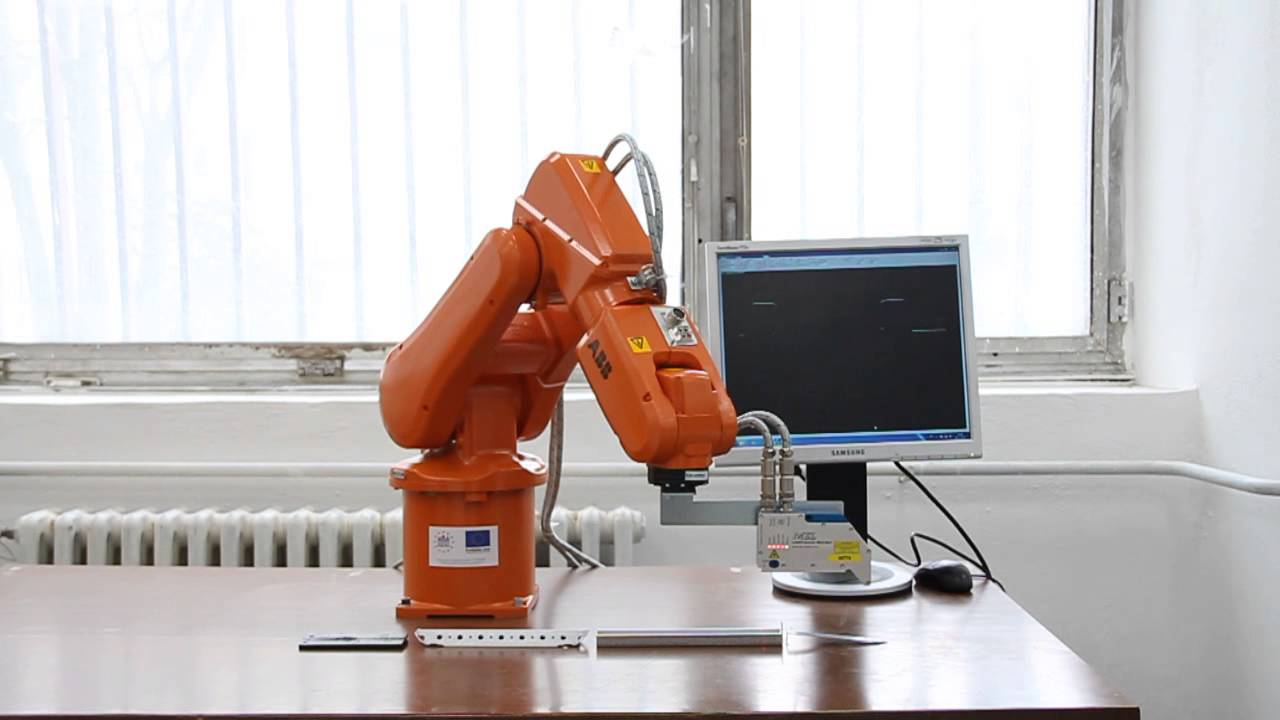
\includegraphics[width=\textwidth]{ABB-irb-120}
\cite{IRB_120}

\subsubsubsection{Universal Robots}
Universal Robots makes two robot arms in this size range. The UR3 is the smaller of the two with a reach of 500mm, payload of 3kg, and 11kg weight. A step up is the UR5 which has a 850mm reach, 5kg payload, and 18.1kg weight. Both of these arms have 6 degrees of freedom. Universal boasts that these arms are easy to implement and re-implement due to compact and lightweight construction, and simple programming interface \cite{RobotWorx}.

\subsubsubsection{KUKA AG}
KUKA makes two robot arms in this size range. The KR3 R540 has a reach of 541mm, payload of 3kg, and weight of 26kg. It can be mounted on the floor, wall, or ceiling for added utility. The K5 sixx R650 is larger with a reach of 650mm, payload of 5kg, and weight of 127kg. It can only be mounted on the floor or ceiling. Both of these arms have 6 degrees of freedom \cite{RobotWorx}.

\subsubsection{Small Industrial Robotic Arm Comparison}
Table \ref{tab:ArmComparisonP} shows a comparison of all the robotic arms discussed in this section.
\begin{table} [H]
	\centering
	\begin{tabular}{| l | c | c | c | c |}
		\hline
		\textbf{Name} & \textbf{Reach (mm)} & \textbf{Payload (kg)} & \textbf{Weight (kg)} & \textbf{Axes} \\
		\hline
		IRB120 & 580 & 3 & 25 & 6 \\
		IRB1200-7/0.7 & 703 & 7 & 52 & 6 \\
		IRB1200-5/0.9 & 901 & 5 & 54 & 6 \\
		UR3 & 500 & 3 & 11 & 6 \\
		UR5 & 850 & 5 & 18.1 & 6 \\
		KR3 R540 & 541 & 3 & 26 & 6 \\
		K5 sixx R650 & 650 & 5 & 127 & 6 \\
		\hline
	\end{tabular}
	\caption{Comparison of $<$1000mm reach industrial robot arms}
	\label{tab:ArmComparisonP}
\end{table}

\subsubsection{Modular Arms}
While there are many industrial arms in production, there are very few modular robotic arms. There is one commercially available robotic arm, the Robolink, made by igus. A few modular robot arms have been developed, including the reconfigurable modular manipulator (RMM), made by TRACLabs \cite{RMM}, and a single joint for the Modular Robotic Arm project MQP at WPI \cite{MRA}.

\subsubsubsection{igus Robolink} 
Robolink is a modular robotic arm kit produced by the plastics manufacturing company igus.  The kit contains parts to make an arm that is up to 6 Degrees of Freedom (DOF), with belt driven linkages powered by stepper motors that reside in the base of the robot.  Robolink offers 7 individual links, ranging from 1-2 DOF and differing based upon their kind of motion (pivoting, rotating, swiveling).  Each link is made of a lightweight and strong plastic or carbon fiber with cables inlaid in them, resulting in a low cost and weight arm.  The cables used to control these links are made of a high strength synthetic fiber with has a tensile strength of 4,000N.  Separating the actuation of each link from the joint allows the arms to be easily maneuverable with its lightweight and strong joints.  \\
\newline
Purchasers of the kit are able to combine the links in different ways, allowing for a flexible, modular solution to robotic arms. Igus also offers their Robolink software for programming articulated arms that facilitates the programming of individual arms through the use of a simple, intuitive control software. The total cost of a kit to make a 6 DOF arm is \$6000, and buying individual links will cost anywhere from \$370 to \$750 per link. While this price may be low cost compared to other arms such as the ABB robotic arm which can cost up to \$200,000 in total, it is still not low enough for either hobbyists or people interested in learning about robotic arms who are prevented from doing so by the high entry cost. In addition to this, the belt system actuating each link requires the user to thread belts attached to the actuators to each link in order to set up the robot. The long assembly time and intricacy also detracts from the idea of modularity because the time involved in switching configurations can inhibit users from really exploring the different workspaces and combinations this kit can create \cite{igus}.  

\subsubsubsection{Reconfigurable Modular Manipulator}
The reconfigurable modular manipulator developed by TRACLabs for NASA is a fully modular 7-DOF robot arm. Each joint and end effector have the same connector that provides power and control lines throughout the arm. Internal power and control circuitry take in these lines and convert them into movement. Joints can be swapped out by hand in a matter of seconds. Joints accept position or velocity data from the central communication lines and store physical characteristics about the joints in memory. This robot arm is not commercially available \cite{RMM}.

\subsubsubsection{Modular Robotic Arm}
This project aimed to close the market gap between inexpensive toy robot arms and expensive professional grade industrial arms. The group aimed to do this by designing a single joint that could be used to assemble a robot arm. Ultimately, a single DOF joint that was heavy, difficult to manufacture, and expensive to produce was designed and constructed. In their future recommendations section, the group stated that the goal of designing a modular robot arm was possible but their design was not the solution \cite{MRA}.

\subsubsection{Our Robotic Arm System}
Our modular robotic arm kit aims to offer a completely different experience compared to existing products and projects. The system maintains a low cost while providing a versatile platform for beginner engineers or rapid prototyping professionals. This is achieved by avoiding expensive proprietary software and subtractive manufacturing; favoring off-the-shelf parts, 3D-printed structures, and freely available software. Providing custom-built software for controlling the arm creates a plug-and-play environment suitable for most any skill level.

% \subsection{Communications}
% We looked at several types of communications for the purposes of controlling our robotic arm. These include serial UART, SPI, I2C, and CAN. 
% \subsubsection{Controller Area Network}
% A controller area network (CAN) is a system for sending data reliably between distinct subsystems with reasonably low danger of transmission errors. CAN buses are widely used in the automotive industry to allow various computerized parts of the car to talk to one another.

% Research begins here?
\subsubsection{Control board}
The control board is meant to be implemented as an independent module that interfaces with a main controller module. Its tasks are to send and receive data from the main controller and control the position of a single motor. As such, the main factors that must be taken into account when designing the control board are methods of measuring joint position and motor torque, as well as communicate with an off-board controller. Motor torque is proportional to motor current. Therefore, the motor torque will be calculated from the measured current through the motor.

\subsubsubsection{Joint Position Detection}
Angular position sensing must be used to determine the joint angle of the motor. There are several commonly used methods of determining angular position, including potentiometers, optical encoders, and Hall effect sensors \cite{Pot_vs_Sensor,Choose_Sensor_Technology,Choose_Position_Sensor}. A comparison of the different angular sensors can be seen in Table \ref{tbl:Angular_pos_sensorsP}. \\
\newline
Potentiometers are very commonly used to measure angular position due to their simple implementation and low cost. In addition to being low cost, potentiometers provide high linearity and accuracy \cite{Choose_Position_Sensor}. Although generall robust, these sensors do not lend themselves well to many, rapid adjustments or mechanical vibrations. Both of these significantly reduce the lifespan of the sensor \cite{Pot_vs_Sensor,Choose_Position_Sensor}. The situations potentiometers excel in are those that require an easily adjustble voltage at low to medium adjustment frequencies, such as settings nobs on control panels or analog reference voltages as trim potentiometers \cite{Pot_vs_Sensor}. \\
\newline
Hall Effect sensors are less commonly used, and consist of a bipolar magnet rotating above a Hall effect sensor with the axis of rotation perpendicular to the plane of the sensor. Since there is no contact between the rotation and the sensor, these types of sensors have very long lifespans \cite{Pot_vs_Sensor}. Unfortunately, these sensors do not provide high resolution since they are susceptible to electromagnetic interference and temperature, and also have some hysteresis \cite{Choose_Position_Sensor}. \\
\newline
Optical encoders are another method of measuring angular position. These sensors consist of a beam of light that shines on a slotted disk so that as the disk rotates, the slots break the light beam. These sensors can have very high resolutions and are resistant to shock and vibrations \cite{Choose_Sensor_Technology}. Like magnetic sensors, these sensors have very long lifespans since there is no mechanical connection on the sensor \cite{Pot_vs_Sensor}. Unfortunately, these sensors are susceptible to foreign particles blocking the light beam from sensing the slots and causing incorrect readings. The most common kind of optical encoder, the Quadrature encoder, does not sense absolute position; it can only read relative position, meaning that a quadrature encoder would need to be combined with some other sensor in order for the robot to be able to sense its joint angles correctly. Other encoders called Absolute Encoders do not have trouble reading absolute position, but they are prohibitively expensive. \cite{Choose_Position_Sensor}. 

\begin{table}[H]
	\begin{center}
		\caption{Comparison of different angular position sensors}
		\label{tbl:Angular_pos_sensorsP}
		\begin{tabular}{ | p{2.4cm} | r | p{1.6cm} | l | l | p{2.5cm} |}
			\hline
			Sensor & Cost & Linearity & Accuracy & Lifespan & Notes
			\\ \hline
			Potentiometer & \$ & Depends on ADC & Moderate & Short & Repeated motion at the same angle can lead to failure
			\\ \hline
			Encoder & \$\$\$ & Very High & Very High & Long & Cheap ones can't sense absolute position
			\\ \hline
			Hall Effect Sensor & \$\$ & High & High & Very Long & Requires special attention to surrounding magnetic fields when mounting
			\\ \hline
		\end{tabular}
	\end{center}
\end{table}

\subsubsubsection{Current Sensing}
Current sensing can be done in many ways. The most common way is by using a shunt resistor and an amplifier. A variant of this method is to use the resistance inherent in the wires or traces as a shunt resistor. Another common method of current sensing is to use a Hall effect sensor \cite{Current_Sensing}. \\
\newline
Shunt resistors are used in either high side or low side configuration. They are simple to integrate, low cost, and capable of measuring both AC and DC currents. The downsides to this method are relatively large insertion loss that increase exponentially with current, large thermal drift that must be compensated for, as well as large system noise from amplification. There are two main implementations of shunt resistors, high side and low side \cite{Current_Sensing}. \\
\newline
Low side current sensing means that the shunt resistor is placed in the return current path. This method is simpler to implement since the voltage on the shunt resistor is with respect to ground, so it can simply be amplified. Some problems exist with this, however, since the resistor separates the current path from ground. In this configuration, the circuitry used to measure the voltage on the shunt resistor will not report a fault if the system experiences a short circuit \cite{Current_Sensing}. \\
\newline 
High side current sensing means that the shunt resistor is placed on the forward current path. This configuration is able to detect short circuit faults, an advantage to using this configuration over low side current sensing. An additional advantage is that the return current path is directly connected to ground. The downside to high side current sensing is that it requires a differential amplifier since the voltage across the shunt resistor is very close to supply voltage. \cite{Current_Sensing}. \\
\newline
Trace resistance sensing is very similar to using a shunt resistor, but there are some slight differences. Since there isn't a way to control the resistance of a copper trace, the system must be calibrated after being assembled. Another key difference is the amount of amplification needed. Copper traces have very low inherent resistance, so a very large amplification must be used. This large gain imposes a limitation on the maximum measurable bandwidth set by the gain bandwidth product of the amplifier \cite{Current_Sensing}. \\
\newline
Hall effect sensors are commonly used to measure current as well. These sensors can measure current intrusively or non-intrusively, as well as in open loop or closed loop configurations. Non-intrusive devices measure current by wrapping wire around a toroid that focuses the magnetic field on a sensor in a break in the ring of the toroid, or placing the Hall effect sensor on top of the current to be measured. These work fairly well, but are very susceptible to noise from magnetic fields upwards of 10cm away. Methods of shielding these sensors exist, but are complicated and expensive to implement. Intrusive sensors route current through the device and measure the generated magnetic field with a Hall effect device near the current path. Open loop applications take the voltage generated on the Hall effect sensor and condition it to whatever output is needed. Closed loop sensors reroute the sensed current to a secondary coil that is used to generate a proportional current to the measured current. This proportional current is then used as feedback to reduce error \cite{Current_Sensing}. \\
\newline
Insertion loss caused by these sensors is very small. Since these sensors measure current by induction, they can only measure current in a specific frequency band, and high currents at high frequencies can cause these devices to overheat. Most of these frequencies are DC to some upper limit determined by the physical characteristics of the sensor, usually around 100kHz. These sensors cannot be used on their own, since they have an inherent voltage offset, called misalignment voltage, and suffer from high thermal drift. Integrated ICs that compensate for these factors are fairly widespread, allowing for very easy integration \cite{Current_Sensing}.

\subsubsubsection{Off-Board Communication}
There are many types of communication protocols that could be used to communicate with the main controller. Common protocols include SPI, I$^2$C, RS232, RS485, and CAN. Of these, SPI and I$^2$C are meant mostly for chip to chip communication while RS232, RS485, and CAN are all meant for module to module communication \cite{SerialCompared}. A comparison of these protocols can be seen in Table \ref{tbl:Comm_CompareP}. \\
\newline
SPI is a full duplex, synchronous serial link consisting of 3 lines, SCLK, MOSI, MISO, and an additional line for every peripheral, CS. Data rates of up to 10MHz or more are possible due to the elimination of addressing with the CS lines and dedicated clock line \cite{SerialCompared}. Using SPI for controller-to-controller communication presents a problem, however. Since the data transfer rate is controller by the master, the slave could fall behind on processing data. This can be avoided by only transmitting data one direction at a time. Typically, SPI is limited to onboard communications since its signal degrades fairly quickly over distance \cite{CANvSPI}. \\
\newline
I$^2$C is a half duplex, synchronous, multi-master bus consisting of a clock and data line. Data rates of up to 3.4MHz can be reached, and each device has a unique address or multiple addresses to avoid overlap. An interesting aspect of I$^2$C is clock stretching. Clock stretching is when a slave pulls the clock low to stall the master until it has enough time to process information. Typically, I$^2$C is limited to onboard communication since its signal degrades fairly quickly over distance \cite{SerialCompared}. \\
\newline
RS232 is a common full duplex interface that consists of two transmitter/receiver pairs. The protocol limits communication to 1 sender and 1 receiver per line. Data rates of up to 115.2KHz are possible at a range of up to 200ft. Data is typically sent in 8N1 format with 8 data bits, no parity bit, and 1 stop bit or 7E1 format with 7 data bits, even parity bit, and 1 stop bit \cite{SerialCompared}. \\
\newline
RS485 is a full duplex multi-master protocol that consists of up to 32 transceivers on the bus. Data transmission rates of up to 10Mbps and distances of up to 4000ft are possible. Transmission can be reduced to half duplex by removing one transceiver at each node. Data is sent much the same as in RS232 with either 8N1 or 7E1 being common formats \cite{SerialCompared}. \\
\newline
CAN is a half duplex multi-master bus protocol that allows for many nodes to connect and send data on the two transmission lines. Messages are sent with unique addresses that also act as arbitration for bus priority. Packets are fully defined with 11 or 29 bit addresses, 0-8 bytes of data, and some additional control and verification bits \cite{CAN_Guide,CAN_Requirements}. Data rates of up to 1MHz and distances of up to 3000ft are possible. Multiple error checks are implemented at the hardware level since packets are predefined, allowing the controller to load a transmit buffer and let the transceiver send a message or wait until a receive buffer is full before reading the message \cite{CANvSPI}. 

\begin{table}[H]
	\begin{center}
		\begin{tabular} {| l | l | p{2cm} | p{2.5cm} | p{2.5cm} |}
			\hline
			Protocol & Max Distance & Max Speed & Wires needed & Notes \\ \hline
			SPI & Within circuit board & 10MHz & SCLK, MOSI, MISO, + 1 CS for each node & No addresses needed
			\\ \hline
			I$^2$C & Within circuit board & 3.4MHz & 2 & Address included in message
			\\ \hline
			RS232 & 200 feet & 115.2KHz & 4 & Can include parity bit
			\\ \hline
			RS485 & 4000 feet & 10Mbps & 4 & Can transmit fast or far but not at same time
			\\ \hline
			CAN & 3000 feet & 1MHz & 2 & Resilient signal
			\\ \hline
		\end{tabular}
	\end{center}
	\caption{Comparison of off-board communication protocol performance}
	\label{tbl:Comm_CompareP}
\end{table}

% \begin{figure}[H]
% \centering
% \includegraphics[width=\textwidth]{Detailed_Block_Diagram}
% \caption{Functional block diagram of the system}
% \label{fig:Functional_Block_Diagram}
% \end{figure}

\subsection{Description of Work}
% Section outline
% Overall summary of section - ~1 sentence per major topic
% ~1 Paragraph for each major topic

% What work is there to be done?
There are many different ways to accomplish the goals we set. We decided to design several "smart" joints, "dumb" sticks of various lengths that passes signals through from joint to joint, changeable end of arm tools, a base for routing messages to each joint as well as providing power to the entire system, and a computer for performing complex real-time calculations. We plan to design every component listed in the kit of parts found in Appendix \ref{app:KitParts}. \\
\newline
We decided on designing two different joints (twist and rotation), with keyed connectors so they can connect in one of four orientations. Two kinds (straight and right angle) and three different lengths (75mm, 150mm, 225mm) of sticks will be designed as well. Joints can connect to sticks and joints, but sticks can only connect to joints. As such, the connectors will have to be designed with this in mind. Each connector will have to make a strong physical connection as well as a solid electrical connection to send power and data through to each Joint. \\
\newline
Each joint will have a control board that allows it to connect to the main communications line running through the system and control the motor on the joint. This board will have all of the necessary components for controlling one motor and communicating with the base. The base will act as an interface between the computer that is performing all of the complex calculations and the joints that are controlling their positions. The computer will need to have a USB port and be able to run Python programs.\\
\newline
We will develop some software for controlling the arm with a GUI that will run on the user's computer. This software will have a simple control interface for moving the arm, and some configurable settings to act as inputs for the kinematics equations. In addition to this we will develop a code library for end users to interface with in their own code.

\subsection{Methodology}
\subsubsection{Kit Components}
We decided to break a robot arm down into its component parts. We came up with the main parts of our kit: sticks, joints, a base, and end of arm tools. This breakdown was to try to maximize modularity while keeping the pieces relatively simple. By separating the joint from the stick, we can have multiple sticks, which are easy to manufacture, of different types and lengths to offset a few types of joints, which are difficult to manufacture. The base is necessary to send and receive computation control from a computer. Multiple end of arm tools are needed to provide functionality to the arm besides movement.

\subsubsection{Connectors}
The connectors are vitally important to the functionality of this project. A good connector will need to make solid mechanical and electrical connection between parts while also providing the ability to quickly connect and disconnect parts. In addition, the type of connection we choose will affect the modularity of the system as a whole. The important things to note while deciding on criteria for the connector are how/if they will be keyed, how they will pass electrical signals, where exactly the connector will be on the joints, and how the connector will be secured.

\subsubsubsection{Connector Position on Joints}
Connector position is the first major design choice we had to make. They can be positioned either on the axis of rotation of the joint or off the axis of rotation of the joint, and selecting one method versus the other vastly changes the way that the connector would work. Putting the connector ON the axis of rotation means that the connector would connect to the joint axis directly, while putting it OFF the axis of rotation means the connector would connect to a piece that is connected to the joint axis. \\
\newline
The advantage that placing the connector off the axis of rotation has over placing the connector on the axis of rotation is that the joint will be a solid unit. Having the joint be a solid unit seems a better design choice than splitting it in half, so we decided to go with putting connectors off the axis of rotation.

\subsubsubsection{Securing the Connection}
%available options: no tools, single screw, multiple screws, slots with removable pins
One of the important aspects of a modular system is how easy it is to connect or disconnect parts to or from that system. The main options for quick connections are requiring no additional hardware, requiring a single screw, and requiring slots and pins. \\
\newline
The most obvious solution is to connect parts with no additional hardware required. This creates a very complicated design challenge since using no tools means the user would have to secure any connection with just their hands. This can weaken the joint mechanically. The advantage to this method has is that it is fairly quick. \\ 
\newline
A step down in the simplicity solution is to require a single screw to join two pieces together. This is still simple and pieces can be connected somewhat quickly, but does require a tool to connect pieces. The main advantage is that screws hold parts together very well and the mechanical integrity of the connection should be held. \\
\newline
Another option is to design the joints and sticks in such a way that they slot together and are held in place with pins. This requires additional hardware, but no tools. This should keep pieces together fairly well while still allowing connections to be made quickly and easily. \\
\newline


\subsubsubsection{Keying the Connector}
Keying the mechanical connection between joints, sticks, and the base changes how modular the system is overall as well as how many unique components will be needed in each kit. Not keying the connection is not an option since this would allow the user to connect the pieces together in any orientation and the orientation needs to be known in order to accurately control the arm. This leaves two main options for the connections: keying for 1 orientation and keying for 4 orientations.\\
\newline
Keying the connectors for 1 orientation means that three different kinds of revolute joint must be design to fully represent the ways a revolute joint can move in 3D space. Essentially, this would mean each different joint would rotate about a different axis relative to the connector axis. The modularity of the kit is impacted quite negatively by doing this, since each joint can only connect in one way and therefore cannot be used where another type of rotation is needed. This design is quite simple, however, since the connectors don't need to be rotationally symmetric about any axis. \\
\newline
Keying the connectors for 4 orientations presents a slightly more challenging design problem, however. The connectors would need to be evenly rotationally symmetric 4 ways about the axis of connection in order for this design to work. 4-way keyed connectors will bring the number of unique joints down from 3 to 2. Doing this does help with the modularity of the design, though, since the rotational joint can be implemented to rotate in either axis perpendicular to the connector axis. A disadvantage of this configuration is an increase in complexity. \\
\newline
Since additional complexity when designing is less important that the overall modularity, we decided to go with a 4-position keyed connection. This allows a single rotational joint and only 1 right angle stick design so that the user can construct many different kinds of arms from these simple parts.

\subsubsubsection{Passing Signals}
% rigid connectors on joints, wires running along outside, wires running through inside that pop out at connector
Connectors also need to pass the power and signal buses through from joint to stick or joint. This can be done in one of a few ways, including: rigid mechanical connectors, loose wires running along the outside of parts, wires running inside of parts, and wires connecting internal bus bars. \\
\newline
Rigid mechanical connectors for passing signals would make connection when parts are connected together. These connections would have to be evenly rotationally symmetric 4 ways about the axis of rotation since the mechanical connectors are. A disadvantage of these connectors is that they rely on the integrity of the mechanical connection to pass electrical signals properly. If the connection flexes or bends too much then the electrical connection could break even though the mechanical connection is still mostly intact. Another disadvantage is that this is the most costly option for passing electrical signals, requiring 4 connectors per connection. \\
\newline
Loose wires along the outside of the parts have several advantages over rigid mechanical connectors. The first of which is that they only require one set of connections per connector. This reduces the cost of each connector significantly. The main disadvantage of this kind of electrical connection is that the wires could get snagged on something since the system is supposed to be active and moving. Another disadvantage is that the wires need to have enough slack to move with the arm without limiting the arm's movement.  \\
\newline
Wires running through the parts that pop out at the connectors is another option or passing signals along the system. This option is practically the same cost as external wires, but doesn't have the problem of wires snagging on the environment. Unfortunately this doesn't solve the problem of wires needing lots of slack to allow for movement of the whole system. \\
\newline
Short wires that connect some internal bus bars provide a more expensive solution to this problem. This would remove the problem of wires needing slack for the entire system. Instead, wires would only have enough slack for one joint. Doing this does bring some complexity issues, however, since the bars would have to be designed into the system and not added on at the end. \\
\newline
For our design we decided to use internal wires running the length of the system. The low cost and simplicity of this solution outweighs the negatives of having to add lots of extra wire to account for movement of the system.\\

\subsubsection{Sticks}
%things to decide for sticks: material, lengths, types (straight, right angle)

Sticks are the things that connect joints together and space joints out. They do not have any electronics on board; they simply pass power and communication wires along to the rest of the arm. They need to be strong, light weight, and inexpensive.\\
\newline
Sticks have an input side and an output side. Two kinds of sticks will need to be created: one will be straight, and one will have a right angle at the input side.

\pagebreak

%yes I like this
%But it makes the page before look so awkward and sad. And it still puts the footnotes too high up


%The following defines two counter variables: startNum and runCount. Every time a new footnote is declared, we increment runCount by 1. Then, when we're populating the footnotes with words, we start with number startNum and count upwards.
\FPeval{\startNum}{(thefootnote)}
\FPeval{\startNum}{round((\startNum) + 1,0)}
\FPeval{\runCount}{\startNum}

\begin{table}[H]
	\begin{center}
		\caption{Comparison of materials to construct sticks}
		\label{tbl:stick_materials}
		\begin{tabular}{ | l | l | p{1.5cm} | p{2.5cm} | p{2.5cm}| l |}
			\hline
			Stick Material & Cost/kg & Cost/ 20mm & Rigidity & Complexity & Weight \\ \hline
			3D-printed PLA\footnotemark[\runCount] & ~\$20/kg & \$3 & Might break  & Low: Very few constraints on possible designs & 150g \footnotemark[\runCount]
			\\ \hline
			\FPeval{\runCount}{round((\runCount)+1,0)}%
			
			PVC\footnotemark[\runCount] & \$7 & \$0.70 & Bends over time & Connect/ Disconnect easily & 106g\\ 
			\hline
			%I would have thought that the next line needed to add 1, not 2. My working hypothesis is that global variables can't really be modified from inside a table. I don't get it. Clearly the line is doing something, or else the \footnotemark line would simply do nothing.
			\FPeval{\runCount}{round((\runCount)+2,0)}%
			
			Carbon Fiber\footnotemark[\runCount] & \$66 & \$6 & Strong, but possibly too thin & & 58g\\ 
			\hline
			%I'm surprised that the next line adds 3 instead of 1. It works this way though. Oh well.
			\FPeval{\runCount}{round((\runCount)+3,0)}%
			
			80/20\footnotemark[\runCount] & \$2.46 & \$2 & Not going anywhere & Nice connecting options & 154g\\ 
			\hline
			%Only needed if more footnotes are added
			%\FPeval{\runCount}{round((\runCount)+1,0)}%
			
		\end{tabular}
		
	\end{center}
\end{table}
\footnotetext[\startNum]{This number assumes 100\% infill. The actual number will almost certainly be lower.}
\FPeval{\startNum}{round((\startNum)+1,0)}

\footnotetext[\startNum]{\url{http://www.homedepot.com/p/Formufit-1-in-x-5-ft-Furniture-Grade-Sch-40-PVC-Pipe-in-White-P001FGP-WH-5/205171542?cm\_mmc=Shopping\%7cTHD\%7cG\%7c0\%7cG-BASE-PLA-D26P-Plumbing\%7c&gclid=Cj0KCQjwx8fOBRD7ARIsAPVq-Nlw\_xbuCOf-QHORvUW4gQ4Dx7SiZt\_vqQ3OvxBdTW-eckQhdp5WWFYaAs9DEALw\_wcB&gclsrc=aw.ds&dclid=CIagtKLB09YCFUuraQodN\_MAOQ}}

\FPeval{\startNum}{round((\startNum)+1,0)}

\footnotetext[\startNum]{\url{https://www.rockwestcomposites.com/45552?gclid=Cj0KCQjwx8fOBRD7ARIsAPVq-NmCNUg6ULxgd9udG-xSuPtJuHKgCLjUSgX\_zXPDgRr2CmKU0tSXX-waAgb9EALw\_wcB}}

\FPeval{\startNum}{round((\startNum)+1,0)}

\footnotetext[\startNum]{\url{https://8020.net/1010.html}}



We choose to use 3D-printed PLA. While it's not the lowest cost option, nor is it the lightest one, its high configurability makes it the ideal material for our needs - especially given its availability for potential customers; anybody with a 3D-printer would be able to make one of our arms. Also, while aesthetic concerns should not be the only factor, we're allowed to consider the way the final product would look. An arm made from PVC would reflect poorly on all the involved parties.


\subsubsection{Motor Selection}
\begin{table}[H]
	\begin{figure}[H]
		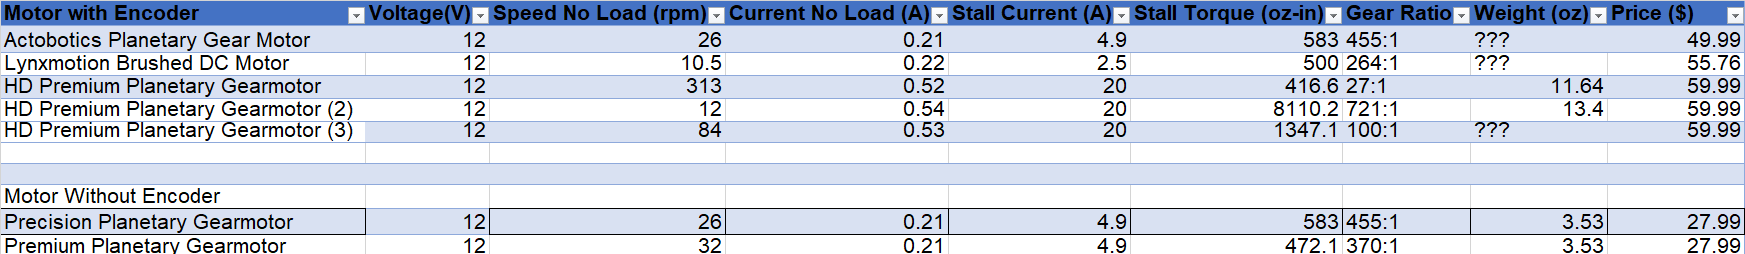
\includegraphics[width=\textwidth]{Pictures/motor_chart}
	\end{figure}
	\caption{Comparison of Possible Motors}
	\label{tbl:Motor_Chart}
\end{table}


To choose our motors, we looked for high-torque, low-cost DC motors. We chose to go with DC Brushed motors to control our arm because they are quiet, low-cost, vibration free and fairly efficient. We also considered using Dc Brushless motors as well as Stepper Motors, but each had their own pros and cons. Brushless motors cost much more than comparable brushed motors, and require complicated control logic to operate. Stepper motors were a good option due to their ability to be backdriven and their built in discrete steps for controlling. But, they do not operate well under conditions where the load changes significantly in a short period of time and also require external control to keep track of the position.  \\
\newline
Once we decided to use brushed DC motors, our next step was to find suitable motors that fit our criteria of high torque and low cost. We found 2 categories of motors that seemed to fill these requirements, planetary gearbox motors and spur gearbox motors. Planetary gearboxes work by having multiple "planet" gears revolving around a central "sun" gear that rotates in place. They are named for their resemblance of the planets orbiting around the sun. All of the "planet" gears are held in place by an outer "ring" gear that acts to keep the "planet" gears in contact with both the "sun" and the "ring". By having these idler gears rotating around a central axis, you can have torque transferred linearly, without the need for offset shafts, greatly reducing the total size of the gearbox. With multiple gears transferring the torque load at one time, the individual load on each tooth is lowered making these perfect for high torque applications. Spur gearboxes on the other hand use linear offset shafts that transfer the entire torque from one gear to the next until the output shaft in a direct chain.  This means that they wear out much faster since the torque load is much higher on individual gears and teeth.  Therefore, since we need a reliable high torque motor, we decided to go with planetary gear motors.  \\
\newline
Once we had made the decision to go with a planetary gearbox brushed DC motor, we made a chart as seen in Table 5 of possible motors that had high stall torques.  One final decision that we had to make was whether or not to purchase a motor with a rotary shaft encoder. Rotary shaft encoders provide easy control over DC motors by relaying the position of the shaft before the gearbox on the motor.  This allows for high resolution control in the case of high gear reductions but also costs a fair amount extra to purchase with the motor.  Considering that the motor is just a part of the joint and we care more about the position of the overall joint rather than the motor itself, we decided to lower cost and go with a less expensive non-encoder motor.  By doing this we are moving the point at which we control the joint system from the motor to the joint if we use an absolute encoder on the joint shaft.  This results in a closed loop control system which is better suited to controlling the arm in our situation and is more cost-effective.  

\subsubsection{Control Board Part selection}
Selecting the types of sensors to use for the control board was a very important step of the control board design. There are many different types of sensors to accomplish each major goal that the control board must accomplish.
\subsubsubsection{Joint Angle Sensor}
Potentiometers seem like a good choice due to their simplicity and high accuracy capabilities. However, they do not lend themselves well to this application because of how quickly they wear out. Over time, as the joints move to different positions, the potentiometers will wear out quickly and cause inaccurate readings. Additionally, long lifespan and high resolution potentiometers can be very expensive. Furthermore, potentiometers are large and can be difficult to mount. Finally, the hard stop on the potentiometer means the joint angles will be limited to a certain range (typically about 270 \textdegree  for single turn potentiometers).\\
\newline
The next obvious solution is to use optical encoders because they will not wear out and offer very high resolution capabilities. These sensors are not well suited for this application, however, since they are typically expensive, especially for high resolution encoders - and ones that are capable of reading absolute position. Additionally these sensors are somewhat bulky and would take up too much space in the closed environment of a joint. \\
\newline
This leaves us with Hall effect sensors. These sensors are very small and moderately high resolution while also being a contact-free sensor, so wearing them out will not be a concern. A main concern with Hall effect sensors is that they need to be mounted somewhat precisely and carefully. Traditional machining methods make this difficult to accomplish, but 3D printing allows us to easily overcome this challenge.  Another concern is external electromagnetic interference, but with somewhat careful circuit board design, we should be able to minimize this issue.

\subsubsubsection{Motor Current Sensor}
A shunt resistor seems practical due to the simplicity of the design, but careful designing must be done in order to get the noise levels down to a reasonable amount. In addition to this, the power loss when using a shunt resistor could cause the arm to stall before anticipated. When the shunt resistor takes power from the motor, the whole motor curve slides inward, decreasing the maximum power output. Trace resistance would be a good alternative, but requires calibration after the circuit is constructed. \\
\newline
Instead of these, we decided to use a Hall effect current sensor. Hall effect current sensors are ready-made sensors that give low noise, properly calibrated outputs, are not very expensive, and are easy to integrate into a circuit design. These sensors have extremely small power losses to the motor. The main drawback of these sensors is that they have a low bandwidth, but we are using DC motors so this should not be a problem. Some care will need to be taken when placing these on the circuit, however, since they are sensitive to external magnetic fields.

\subsubsubsection{Off-board Communication}
SPI and I$^2$C are mostly used for on-board, controller-to-peripheral communications and therefore are not a good choice for the base to control board communication. RS232 is not a good solution for this problem either because it is a single transmitter and single receiver per line. This leaves RS485 and CAN. \\
\newline
RS485 and CAN are similar in many ways, but with a few key differences that separate them. RS485 is very fast to transmit and simple to implement, but takes a lot of the controller's time to send packets. CAN has the advantage because the controller and transceiver control the transmission independent of the controller so the controller has more free time to process data. Another advantage CAN has over RS485 is the amount of error checking that goes on to ensure proper message transmission. For these reasons, we decided to use CAN to communicate between the base and control boards.
% TYPES: SPI, I2C, RS232, RS485, CAN

\subsubsection{Arm Structure}
Arm structure is not something we wanted to define, since the end user is supposed to create their own arms, but there were some basic things we needed to define. The first of these is that every arm must begin with a base and end with an end effector. This is because the central CAN bus must be terminated with resistors at both ends. An alternative to this is to have every piece terminate the CAN bus if it is the last piece in the chain, but this creates unnecessary complexity in each piece. The second constraint placed on arm construction is that sticks cannot connect to other sticks. This is because we didn't want the user to construct an arm with ridiculous length that would be impossible to lift.

\subsubsection{Arm Base}
% Talk about requirements for base
% take in new joint data at certain speeds
% output new joint data at certain speeds

\subsubsection{End-of-Arm Tooling}


\subsection{Constraints}
% This section is most likely going to be pretty sparse

Budget will likely be the biggest constraint with this project. The stipend given to students by WPI may not cover all of the costs incurred when constructing this robot, and the rest will be paid out of pocket by the student team. Another large constraint will be access to a 3D printer for prototyping. It will be crucial to start prototyping early to accomplish all of the design goals. Time will also be a major concern, since there are many time consuming aspects to this project.

\subsection{Acceptance Criteria}
Acceptance criteria for this project will be broken into 5 major categories: Sticks, Joints, End effector, Base, Software application, Code library

\subsubsection{Sticks}
\begin{itemize}
	\item Pass power and signal buses
	\item Strong mechanical connection
	\item 4-position keyed connection
	\item 1 input and 1 output connector
	\item Two kinds of sticks: Straight and Right Angle
	\item Quick to connect and disconnect
	\item Connect to joints but not sticks
	\item Limits exposed wires
\end{itemize}

\subsubsection{Joints}
\begin{itemize}
	\item Receive initialization information and joint angles from base
	\item Moves to joint angles
	\item Send position updates back to base
	\item Pass power and signal buses
	\item Capable of powering logic without powering motors
	\item Control board is the same for each joint (address is selected with DIP switch or in firmware)
	\item 4 position keyed connection
	\item 1 input and 1 output connector
	\item Quick to connect and disconnect
	\item Connects to joints and sticks
	\item Limits exposed wires
\end{itemize}

\subsubsection{End Effector}
\begin{itemize}
	\item Receives power and signal buses
	\item 4 position keyed connection
	\item 1 input connector
	\item Quick to connect and disconnect
	\item Connects to joints but not sticks
	\item Limited exposed wires
\end{itemize}

\subsubsection{Base}
\begin{itemize}
	\item Sends and receives joint angles to/from personal computer
	\item Receives initialization information from computer, then sends it to all joints on signal bus
	\item Outputs power and signal buses
	\item Converts AC wall power to system power bus
	\item Power supply and arm on/off switch
	\item Capable of powering logic without powering motors
	\item Array of indicator LEDs
	\item 4 position keyed connection
	\item 1 output connector
	\item Quick to connect and disconnect
	\item Connects to joints and sticks
	\item Limits exposed wires
\end{itemize}

\subsubsection{Software Application}
\begin{itemize}
	\item Sends configuration information to Code Library
	\item Sends individual joint angles or pose commands to robot through Code Library
	\item GUI to adjust current arm configuration parameters
	\item Record and play back sequence of poses
	\item Acts as a front-end for code library
	\item Stretch goal: 3D model of arm moving in real-time
\end{itemize}

\subsubsection{Code Library}
\begin{itemize}
	\item Written so that it can interface with multiple languages
	\item Receive configuration information from user, selects control constants, sends to base
	\item Able to control the robot: Receive joint status, send joint angles
	\item Calculate joint angles using kinematics
\end{itemize}

\subsection{Kit Components}
\label{app:KitParts}
\begin{itemize}
	\item 3x Twist Joints (axis of rotation parallel to input Stick)
	\item 6x Rotational Joints (axis of rotation perpendicular to input Stick)
	\item 3x 75mm Straight Sticks
	\item 3x 150mm Straight Sticks
	\item 3x 225mm Straight Sticks
	\item 3x 75mm Right Angle Sticks
	\item 3x 150mm Right Angle Sticks
	\item 3x 225mm Right Angle Sticks
	\item 1x Claw Gripper End-of-Arm Tool
	\item 1x Hook End-of-Arm Tool
	\item 1x Capacitive Stylus/Pointer End-of-Arm Tool
	\item 1x Arm Base
	\item Stretch Goals:
	\begin{itemize}
		\item Prismatic Joint(s)
		\item 1x Universal Gripper End-of-Arm Tool
	\end{itemize}
\end{itemize}